\documentclass[a4paper,11pt]{article}
\usepackage[utf8]{inputenc}
\usepackage{geometry}
\geometry{left = 4.0cm, right = 4.0cm, top = 4.0cm, bottom = 3.5cm}
\usepackage[onehalfspacing]{setspace} 
\usepackage{graphicx}
\usepackage{tabularx}
\usepackage{hyperref}
\usepackage{float} 
\usepackage{ragged2e} %%blocksatz \justifing
\usepackage{minted}
\usepackage[english]{babel} % 将语言改为英文
\usepackage[babel,english=american]{csquotes} % 设置英文引号样式
\usepackage[backend=biber, style=apa]{biblatex} 
\newcommand{\showfontsize}{{\f@size pt}}
% \addbibresource{literature.bib}
\setlength{\bibitemsep}{1em}

%%%%%%%%%%%%%%%%%%%%%%%%%%%%%%%%%%%%%%%%%%%%%%%%%%%%%%
% Title Page
%%%%%%%%%%%%%%%%%%%%%%%%%%%%%%%%%%%%%%%%%%%%%%%%%%%%%%%
\documentclass{article}
\usepackage[utf8]{inputenc}
\usepackage[a4paper, margin=1in]{geometry}
\usepackage{titling} 

% 设置标题页格式
\pretitle{\begin{center}\Huge\bfseries}
\posttitle{\par\end{center}\vspace{2cm}}
\preauthor{\begin{center}\Large}
\postauthor{\par\end{center}\vspace{2cm}}
\predate{\begin{center}\Large}
\postdate{\par\end{center}}

% 计算垂直间距使内容均匀分布
\renewcommand{\maketitlehooka}{%
  \setlength{\droptitle}{-5cm} % 调整标题起始位置
  \vspace*{\fill} % 顶部填充
}
\renewcommand{\maketitlehookd}{%
  \vspace*{\fill} % 底部填充
}

\begin{document}

\title{COMP3314 Assignment 3 \\ Image Classification Report}
\author{
    Team name: 99\% \\
    \vspace{0.5cm} 
    Chen Yuxuan \\
    Li Yufei \\
    Liu Yantong 3036127012
}
\date{\today}

\maketitle
\newpage
%%%%%%%%%%%%%%%%%%%%%%%%%%%%%%%%%%%%%%%%%%%%%%%%%%%%
% Table of Contents
%%%%%%%%%%%%%%%%%%%%%%%%%%%%%%%%%%%%%%%%%%%%%%%%%%%%%
\tableofcontents\newpage
%%%%%%%%%%%%%%%%%%%%%%%%%%%%%%%%%%%%%%%%%%%%%%%%%%%
% Abstract
%%%%%%%%%%%%%%%%%%%%%%%%%%%%%%%%%%%%%%%%%%%%%%%%%%%
\section{Abstract}


%%%%%%%%%%%%%%%%%%%%%%%%%%%%%%%%%%%%%%%%%%%%%%%%%%%
% Dataset Analysis
%%%%%%%%%%%%%%%%%%%%%%%%%%%%%%%%%%%%%%%%%%%%%%%%%%%
\section{Dataset Analysis}
In this section, we present an overview of the dataset, analyzing the statistics on the number of categories. Additionally, we will visualize representative examples from each category to illustrate the diversity and characteristics inherent within the dataset. This analysis aims to provide a foundational understanding of the dataset's structure, which is essential for subsequent modeling and interpretation.

\subsection{Load Data}
We load the data and subsequently convert both the training and testing datasets into NumPy arrays, which are easier for our model to process.

\begin{listing}[!ht]
\begin{minted}{python}
csv_path, csv_test_path = "./data/train.csv", "./data/test.csv"
img_dir, img_dir_test = "./data/train_ims", "./data/test_ims"
data_train = pd.read_csv(csv_path)
data_test = pd.read_csv(csv_test_path)
X_train, y_train, X_test, y_test = [], [], [], []

for _, row in data_train.iterrows():
    img_path = os.path.join(img_dir, row.iloc[0])
    label = int(row.iloc[1])
    img = Image.open(img_path).convert("RGB")
    img = np.array(img).flatten()
    X_train.append(img)
    y_train.append(label)

for _, row in data_test.iterrows():
    img_path = os.path.join(img_dir_test, row.iloc[0])
    label = int(row.iloc[1])
    img = Image.open(img_path).convert("RGB")
    img = np.array(img).flatten()
    X_test.append(img)
    y_test.append(label)

X_train, y_train = np.array(X_train), np.array(y_train)
X_test, y_test = np.array(X_test), np.array(y_test)
X_train_flatten = X_train.reshape(X_train.shape[0], -1)
X_test_flatten = X_test.reshape(X_test.shape[0], -1)
\end{minted}
\caption{Load Data}
\label{listing:python}
\end{listing}

\subsection{Statistics on the number of categories}

\subsubsection{Dataset Size}

\begin{listing}[!ht]
\begin{minted}{python}
print("The shape of the training set: ", X_train.shape)
print("The shape of the testing set: ", X_test.shape)
print("Training set (flattened): ", X_train_flatten.shape)
print("Testing set (flattened): ", X_test_flatten.shape)
print("The size of the label of the training set: ", y_train.shape)
print("The size of the label of the testing set: ", y_test.shape)
\end{minted}
\caption{Print the shape of the datasets}
\label{listing:python}
\end{listing}

\begin{itemize}
    \item \textbf{Size Statistics}
    \item The shape of the training set: \textbf{(50000, 32, 32, 3)}
    \item The shape of the testing set: \textbf{(10000, 32, 32, 3)}
    \item Training set (flattened): \textbf{(50000, 3072)}
    \item Testing set (flattened): \textbf{(10000, 3072)}
    \item The size of the label of the training set:  \textbf{(50000,)}
    \item The size of the label of the test set: \textbf{(10000,)}
\end{itemize}

\subsubsection{Category Label Count}

\begin{listing}[!ht]
\begin{minted}{python}
# Count the labels
count_labels = np.unique(y_train, return_counts=True)

# Create DataFrame
label_counts_df = pd.DataFrame({
    "Label": count_labels[0],
    "Count": count_labels[1]
}).set_index("Label")

# Print DataFrame
print("Count of each label:")
print(label_counts_df)
\end{minted}
\caption{Count the number of each category}
\label{listing:python}
\end{listing}

\begin{table}[h]
    \centering
    \begin{tabular}{|c|c|c|c|c|}
        \hline
        Label 0 & Label 1 & Label 2 & Label 3 & Label 4 \\
        \hline
        \textbf{5038} & \textbf{5016} & \textbf{5032} & \textbf{4991} & \textbf{4982} \\
        \hline
        Label 5 & Label 6 & Label 7 & Label 8 & Label 9 \\
        \hline
        \textbf{4967} & \textbf{4985} & \textbf{4998} & \textbf{5002} & \textbf{4989} \\
        \hline
    \end{tabular}
    \caption{Label Counts in training set}
    \label{tab:example}
\end{table}

\begin{figure}[H]
    \centering
    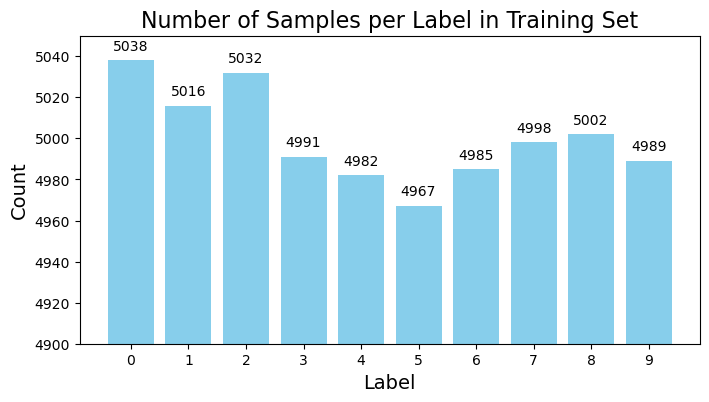
\includegraphics[scale=0.7]{./img/Label_counts.png}
    \caption[Label count] {Label Counts in training set}
\end{figure}

\subsubsection{Other Statistics}

\begin{listing}[!ht]
\begin{minted}{python}
print("Other Statistics for the training set label:")
print(pd.Series(y_train).describe())
\end{minted}
\caption{Print other statistics of the labels of the training set}
\label{listing:python}
\end{listing}

\begin{verbatim}
count    50000.00000
mean         4.49258
std          2.87539
min          0.00000
25%          2.00000
50%          4.00000
75%          7.00000
max          9.00000
\end{verbatim}

\subsection{Image Visualization}
\subsubsection{One Example for Each Category}

\begin{listing}[!ht]
\begin{minted}{python}
def visualize_images_by_label(img_dir, data, y):
    unique_labels = np.unique(y)
    fig, axes = plt.subplots(2, 5, figsize=(15, 6))
    for i, label in enumerate(unique_labels[:10]): 
        indices = np.where(y == label)[0]
        idx = np.random.choice(indices)
        img = Image.open(os.path.join(img_dir, data.iloc[idx, 0]))
        row = i // 5
        col = i % 5
        ax = axes[row, col] 
        ax.imshow(img)
        ax.set_title(f"Label {label}")
        ax.axis('off')
    for j in range(i+1, 10):
        row = j // 5
        col = j % 5
        axes[row, col].axis('off')
    plt.tight_layout()
    plt.savefig("1 example.png", format='png', bbox_inches='tight')
    plt.show()
visualize_images_by_label(img_dir, data_train, y_train)
\end{minted}
\label{listing:python}
\end{listing}

\begin{figure}[H]
    \centering
    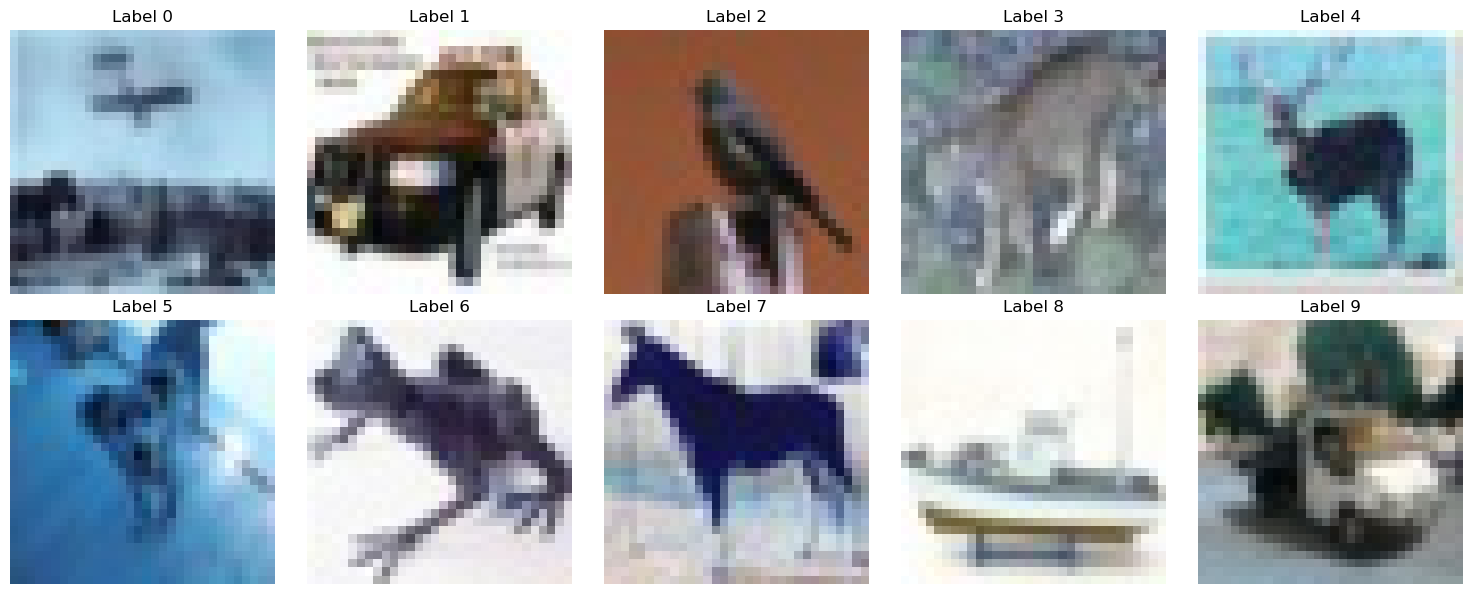
\includegraphics[width=\linewidth]{./img/1 example.png}
    \caption[Label count]{Visualization of one example for each category}
    \label{fig:example}
\end{figure}

\subsubsection{Ten Examples for Each Category}
\begin{listing}[!ht]
\begin{minted}{python}
count_labels = np.unique(y_train, return_counts=True)
label_counts_df = pd.DataFrame({
    "Label": count_labels[0],
    "Count": count_labels[1]
}).set_index("Label")

def get_example_images(label, num_examples=10):
    indices = np.where(y_train == label)[0]
    selected_indices = np.random.choice(indices, 
        size=min(num_examples, len(indices)), replace=False)
    example_images = [os.path.join(img_dir, data_train.iloc[i, 0]) 
        for i in selected_indices]
    return " ".join([f'<img src="{img}" width="50" />' 
        for img in example_images])

label_counts_df["Example Images"] =                               
label_counts_df.index.map(get_example_images)
HTML(label_counts_df.to_html(escape=False))
\end{minted}
\label{listing:python}
\end{listing}

\begin{figure}[H]
    \centering
    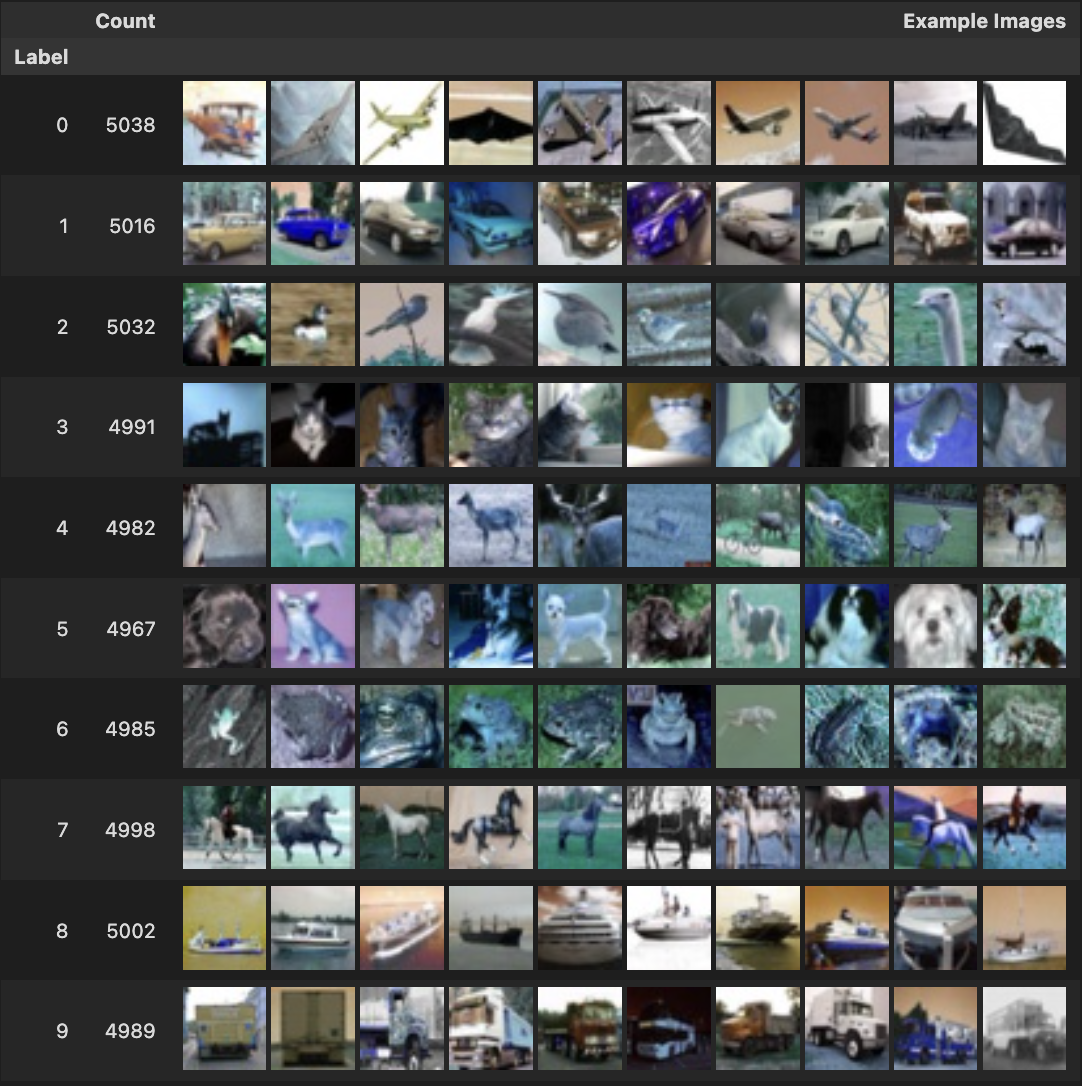
\includegraphics[width=\linewidth]{./img/10 examples.png}
    \caption[Label count]{Visualization of ten example for each category}
    \label{fig:example}
\end{figure}

%%%%%%%%%%%%%%%%%%%%%%%%%%%%%%%%%%%%%%%%%%%%%%%%%%%
% Image Preprocessing
%%%%%%%%%%%%%%%%%%%%%%%%%%%%%%%%%%%%%%%%%%%%%%%%%%%
\section{Image Preprocessing}
TBD

\subsection{Image Resizing}
TBD

\subsection{Feature Extraction}
TBD

%%%%%%%%%%%%%%%%%%%%%%%%%%%%%%%%%%%%%%%%%%%%%%%%%%%%
% Model Training
%%%%%%%%%%%%%%%%%%%%%%%%%%%%%%%%%%%%%%%%%%%%%%%%%%%%%
\section{Model Training}
TBD

\subsection{Model 1}
TBD

\subsection{Model 2}
TBD

\subsection{Model 3}
TBD

% Python code example
\begin{listing}[!ht]
\begin{minted}{python}
def add(x,y):
    res = x + y
    printf("{x} + {y} = {res}")
    return res

x = 3
y = 2
r = add(x,y)
print(r)
\end{minted}
\caption{Python sample code}
\label{listing:python}
\end{listing}

% Image example
\begin{figure}[H]
    \centering
    
\includegraphics[scale=0.7]{./img/nailong.jpg}
    \caption[nailong] {woshinailong}
\end{figure}

%%%%%%%%%%%%%%%%%%%%%%%%%%%%%%%%%%%%%%%%%%%%%%%%%%%%
% Results
%%%%%%%%%%%%%%%%%%%%%%%%%%%%%%%%%%%%%%%%%%%%%%%%%%%%%
\section{Results}
TBD

\end{document}